\section{Overall Approach}

This section presents our approach to realize the decomposition and collaboration for complex industrial control system.
% Industrial Modelling Collaboration Language (IMCL)

\subsection{The Syntax of $IMCL$}
\emph{IMCL} is an event-triggered language. The event trigger is a system running mechanism that the processing of some function waiting for the event triggers and then execute the corresponding operation of this event. Here, we will introduce the abstract syntactic of \emph{IMCL}.
% ������ֵ
\begin{equation*}
    \begin{aligned}
        A_{exp} ::= &\ val \mid X \mid a_{0} + a_{1} \mid a_{0} - a_{1} \mid a_{0} * a_{1} \mid a_{0} / a_{1} \\
        B_{exp} ::= &\ \top \mid \bot \mid a_{0} = a_{1} \mid a_{0} \neq a_{1} \mid a_{0} > a_{1} \mid a_{0} < a_{1} \\
        C_{exp} ::= &\ channel!m \mid channel?m \mid sync.n \\
        E_{exp} ::= &\ E_{0};E_{1} \mid E_{0} \triangleleft b \triangleright E_{1} \mid b * E \mid X := a \mid C_{exp} \\
                    &\mid a \gg Dev \mid a \ll Dev \\
        T_{exp} ::= &\ trigger \ b \diamond E \mid trigger \ channel?m \diamond E  \\
    \end{aligned}
\end{equation*}

$A_{exp}$ is the arithmetic expression where $val$ is value, $X$ is variable, $a_{0}, a_{1} \in A_{exp}$.
$B_{exp}$ is the boolean expression, where $\top$ and $\bot$ are signifying the \emph{true} and \emph{false}. For every \emph{b} $\in$ $B_{exp}$, it is a bool expression. Next, we mainly introduce some specially expression in \emph{IMCL}. $C_{exp}$ is the communication expression. The $channel!m$ signifies sending a value $m$ from a $channel$ . The $channel?m$ signifies receiving a value $m$ from a $channel$. The $sync.n$ means to get the synchronous data $n$.
$E_{exp}$ is the execution expression. Condition choice $E_{0} \triangleleft b \triangleright E_{1}$ is that if $b$ is true then $E_{0}$, else $E_{1}$. The $b * E$ indicates that the $E$ will iterates until $b$ is false. Specifically, $a \gg Dev$ denotes that system transmit value $a$ to physical device $Dev$, while $Dev \ll a$ is getting $a$ from $Dev$. $T_{exp}$ is the event-triggered expression. The $trigger \ b \diamond E$ denotes an event $E$ happens when the $b$ is true. The $ trigger \ channel?m \diamond E_{exp}$ indicates that when receiving a $m$ from the $channel$, the event $E$ will begin to execute.

%\subsection{Modelling the Industrial System Using IMCL}
\subsection{\emph{IMCL} Model for Industrial Control System}

The modeling process focuses on system functions and features as following two steps:

\textbf{Modeling the physical resources. }
Representations of physical resources are different based on diverse industrial environment, for instance, sensors, read-write devices, and the other resources. Considering their effects on the whole system, we describe all those resources as variables to unifying definition of resources.

\textbf{Modeling the system. }
Observing its behavior, the nature of the system is gathering functions, read-write operations, and other actions together. Similar to physical resources, we model them as execution expressions. Multiple execution expressions in one specific order can make up one trigger event marked as $T$.

An \emph{IMCL} model consists of multiple concurrent trigger events, and every event is triggered only when its condition is satisfied. Let $\bowtie$ be the concurrent operation of two events such that $T_1\bowtie T_2$. Then, the \emph{IMCL} model \emph{Prog} can be defined:
\begin{displaymath}
Prog = \overset{n}{\underset{i=1}{\bowtie}} T_{i}, n \in N^{+}
\end{displaymath}


For a given \emph{IMCL} program $Prog_{ori}$, we can get an AST(Abstract Syntax Tree) which contains details of its statements by an open source grammar parser tool, ANTLR.
Then, we can get the corresponding CFG(Control Flow Graph) and DFG(Data Flow Graph) based on AST.

A $CFG = \langle N, E \rangle$ is a directed graph, where \emph{N} is a set of nodes, and $E \subseteq N \times N$ is the set of edges while \emph{DFG} is a data-flow digraph structure. If $(n_1,n_2) \in E$, then $n_2$ is an immediate successor of $n_1$.

During the construction of CFG, we can get the information of each node. For each node $n$, we can have the following three sets: \emph{REF(n)}, \emph{DEF(n)} and \emph{INFL(n)}. \emph{REF(n)} is the set of variables whose values are used at n, and \emph{DEF(n)} is the set of variables whose values are changed at n. \emph{INFL(n)} is the set of nodes transitively control dependence on $n$, and it will not be empty only when $n$ has more than one immediate successor(for example, $n$ is a branch statement or a loop node).

There is a \emph{post} data-dependency($DD_{post}$) set of nodes for every node in the DFG, which is described as follow:\\
\begin{displaymath}
    \forall x \in DD_{post}(n), \ REF(x) \cap DEF(n) \neq \emptyset
\end{displaymath}
The $DD_{post}$(n) denotes that there are some nodes that are all data-depended on node $n$.
% For example, $DD_{post}(m) = \{2,6\}$, which means that at least one variable in both statement 2 and 6 are depended on statement $m$, respectively.

\textbf{SDG:} \ The \emph{System Dependence Graph}(SDG), a graph representation of system model with data dependence and control dependence, and which is based on \emph{CFG} and \emph{DFG}:
\begin{displaymath}
    SDG :=  \bigcup_{i=1}^{N} (CFG \oplus DD_{post}(i))
\end{displaymath}
which denotes that the SDG is a combination of CFG and all $DD_{post}$(i) that data-depended on every statement.

\begin{figure}[!ht]
    \centering
        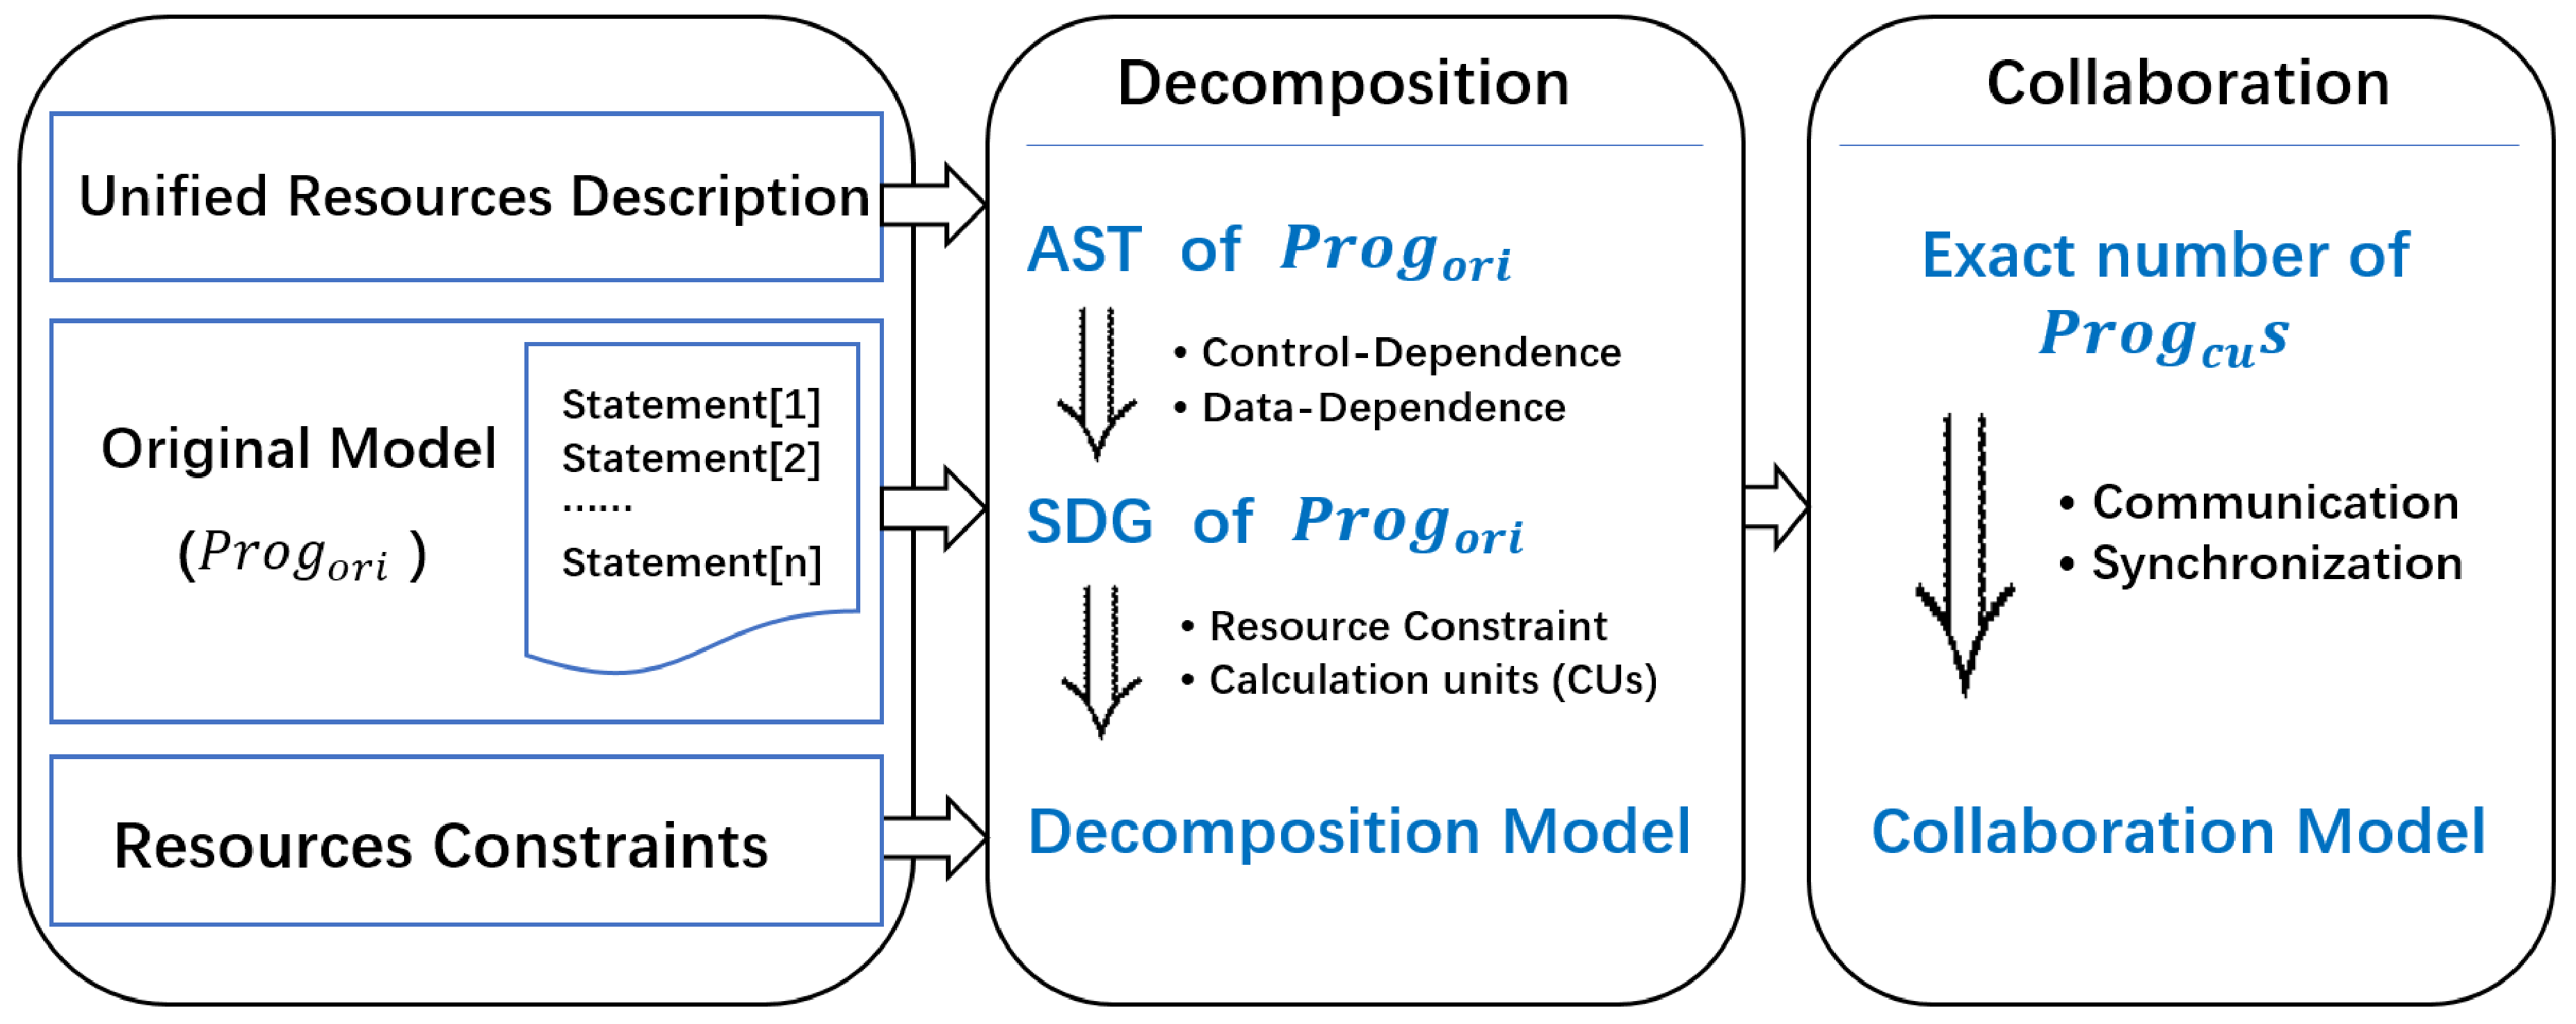
\includegraphics[height=1.5in, width=3.5in]{fig_Approach}
    \caption{Overview of approach for decomposition and collaboration }\label{fig_approach}
\end{figure}

Fig \ref{fig_approach} is the overview of the approach for decomposition and collaboration that we have implemented in our tool.
There are five basic terms for approach:
\begin{itemize}
  \item \textbf{Original Model:}\  The Original model is an \emph{IMCL} model $Prog_{ori}$ given at the beginning time, which is the description of an industrial control system.
  \item \textbf{Statement:}\ The $statement$ is the minimum computational task level for the program. Therefore, the $Prog_{ori}$ can be treated as a set of statements.
  \item \textbf{Resource Constraints:}\ It describes the constraints that physical resources are limited available for specific CUs.
  \item \textbf{Decomposition Model:}\  It is the multiple models that all of the statements in \emph{Original Model} are decompose to specified $CU$. In other words, it is transformed from a $Prog_{ori}$ with the resource constraint to the set of $Prog_{cu}$ for every \emph{CU}.
  \item \textbf{Collaboration Model:}\  Which is a set of the $Prog_{cu}$ interact with each other with communication and synchronization.
\end{itemize}

For one industrial control system, we model the physical resources and system as one \emph{Original Model} ($Prog_{ori}$) . Based on the SDG of $Prog_{ori}$, we can decompose the \emph{Original Model} to the \emph{Collaboration Model} with the resource constraints.
Only with the analysis of SDG, we can determinate the dependence of control flow and data flow to keep the constancy of \emph{Original Model} and \emph{Decomposition Model}.
%As a result, SDG analysis is a very important part of the decomposition.
To decompose the \emph{Original Model} into \emph{Decomposition Model} with resource constraints. $DD_{pre}$, the \emph{pre} data-dependency for each statement, can be obtained from corresponding $DD_{post}$. The definition is as follows:
\begin{displaymath}
    DD_{pre}(j) \ = \ \{ i \ | \ j \in DD_{post}(i), \ \forall i, j \in N \}
\end{displaymath}
where $j$ is a statement that data-depended on the statement in $DD_{pre}(j)$.
% For example, $DD_{pre}(j) = \{2, 7\}$ means that the statement $j$ are data-depended on statement $2$ and $7$.

The key to ensuring the reliability of \emph{Original Model} and \emph{Collaboration Model} is the communication in the process of collaboration, which is based on the SDG analysis.
We abstract the communication protocols between multiple models. The $IMCL$  unifies the communication and data synchronous among multiple models. There are three specific communication methods as follows:
\begin{itemize}
  \item \textbf{CHANNEL.CD!x} and \textbf{CHANNEL.CD?x},  the symbol \emph{CHANNEL.CD} is used for the control message and applied to the communication with control-dependence in multiple CUs or multiple internal event triggers in a signal CU. \emph{CHANNEL.CD!x} shows the model transmits a control message $x$ along the channel; \emph{CHANNEL.CD?x} denotes that receives the control message $x$ via the channel.
  \item \textbf{CHANNEL.DD!x:data} and \textbf{CHANNEL.DD?x:data},  \emph{CHANNEL.DD} is used for data message and is applied to the communication with data-dependence in multiple CUs or multiple internal triggers in a signal CU. \emph{CHANNEL.DD!x:data} shows the model transmits a data message $x$ with $data$ along the channel; \emph{CHANNEL.DD?x:data} denotes that a control message x with data via the channel.
  \item \textbf{SYNC.DATA:data},  the \emph{SYNC.DATA} is used to synchronize the data in different event triggers. Both \emph{CHANEL.DD} and \emph{SYNC.DATA} are used to synchronize the data. But different from \emph{CHANEL.DD}, \emph{SYNC.DATA} does no have any dependence on the $data$ in the original Model.
\end{itemize}
